%!TEX root = ../../report.tex

\begin{figure}[!b]
    \centering
    
    % Setup box for subfigure
    \subcaptionbox[Short Subcaption] 
        % Subcaption and label for subfigure
        {Initial state of a particle filter. The particles are randomly spread throughout the entire map and the best guess of the robot position is a random ''cluster'' of particles. \label{subfig:demo1}}
        % Size of figure and subcaption width
        [0.45\textwidth]
        % Figure to include (width should match the above width
        {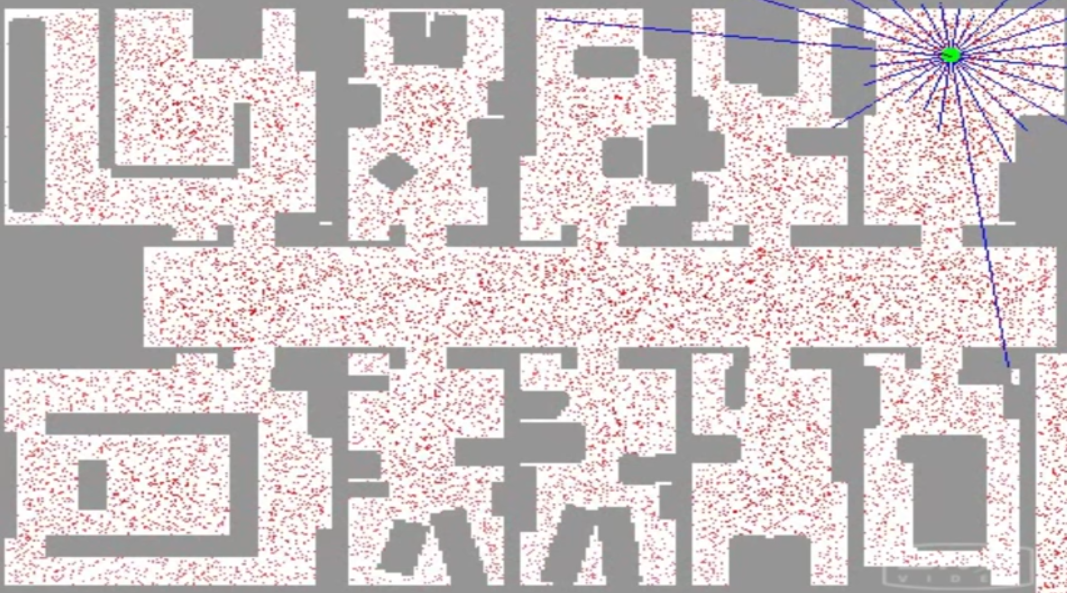
\includegraphics[width=0.45\textwidth]{ParticleFilter/demo1.png}}
%
\hspace{0.02\textwidth} % Seperation
%
    % Setup box for subfigure
    \subcaptionbox[Short Subcaption]
        % Subcaption and label for subfigure
        {After a few measurements, movements and resamples we begin to see a few particle clusters forming. The robot now believes that it is located in the corridor, but is still not quite sure where exactly. \label{subfig:demo2}}
        % Size of figure and subcaption width
        [0.45\textwidth]
        % Figure to include (width should match the above width
        {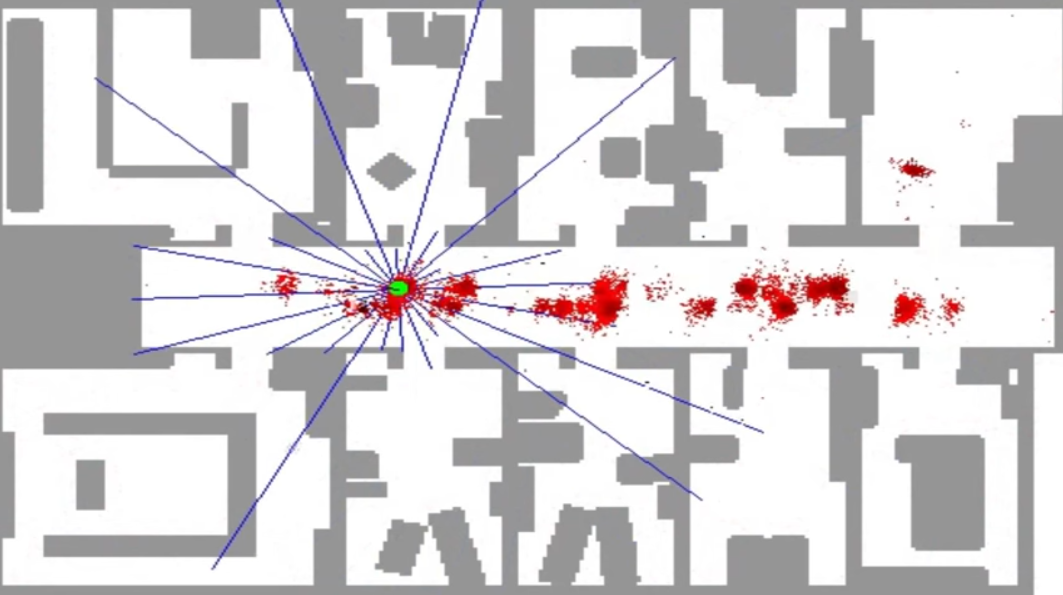
\includegraphics[width=0.45\textwidth]{ParticleFilter/demo3.png}}%
%
\\ % Seperation
%
    % Setup box for subfigure
    \subcaptionbox[Short Subcaption]
        % Subcaption and label for subfigure
        {As the robot continuously measure, move and resample it narrows down the possible positions. Here we see two particle clusters with quite strong beliefs, but the robot is still unable to tell exactly which cluster is the right one, due to the symmetry of the corridor.\label{subfig:demo3}}
        % Size of figure and subcaption width
        [0.45\textwidth]
        % Figure to include (width should match the above width
        {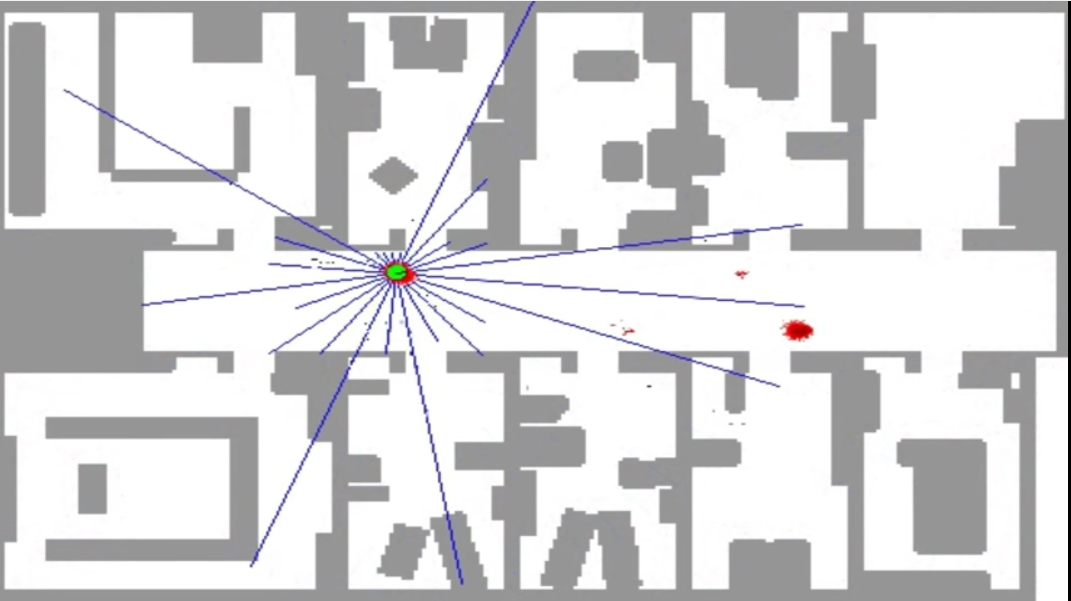
\includegraphics[width=0.45\textwidth]{ParticleFilter/demo4.png}}
%
\hspace{0.02\textwidth} % Seperation
%
    % Setup box for subfigure
    \subcaptionbox[Short Subcaption]
        % Subcaption and label for subfigure
        {When to robot enters a room, it is able to differentiate the rooms from each other and thus eliminate the incorrect belief of the other particle cluster, ending up with one good approximation to the actual position in the map. \label{subfig:demo4}}
        % Size of figure and subcaption width
        [0.45\textwidth]
        % Figure to include (width should match the above width
        {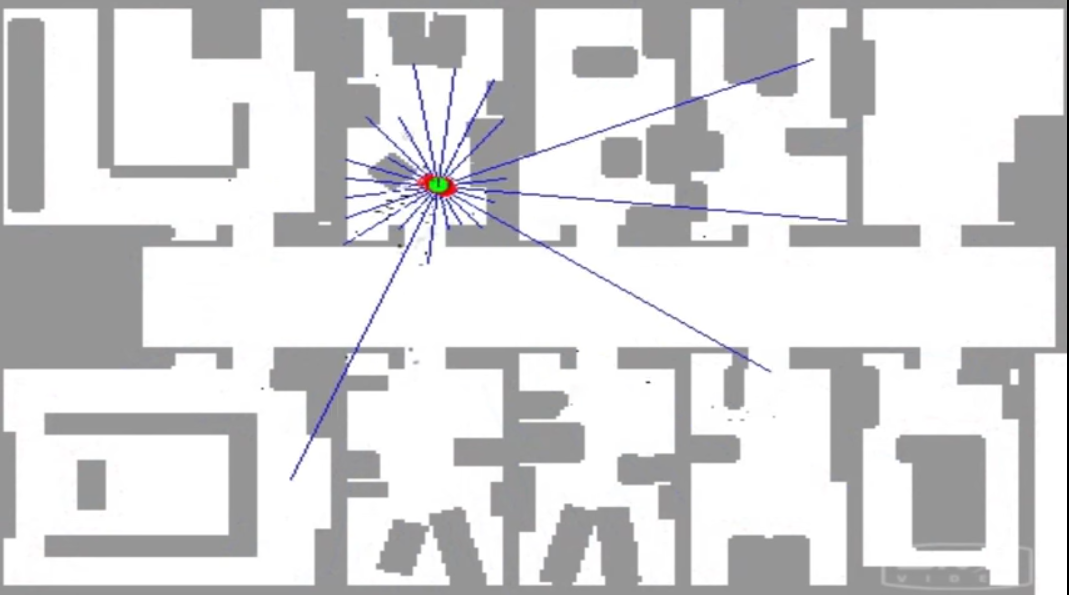
\includegraphics[width=0.45\textwidth]{ParticleFilter/demo5.png}}

    % Caption and label of whole figure set
    \caption[Short Caption]{Illustration of global localization using a particle filter. The map is a corridor and multiple rooms, where the white areas are accessible and the grey areas are walls, furniture etc. Each red dot represents a particle and the green circle represents the best guess of the robots position at each specific time.}
    \label{fig:particleDemo}
\end{figure}